\documentclass[a4paper]{article}

\usepackage{xcolor,hyperref,mdframed,pdfpages}
\usepackage[top=6cm]{geometry}
\usepackage{titlesec}
\usepackage{tablefootnote,subcaption}

\usepackage[pages=all]{background}

\backgroundsetup{
	scale=1,
	color=black,
	opacity=1.0,
	angle=0,
	contents={
\includegraphics[width=\paperwidth,height=\paperheight]{Background.jpg}}
}

% Format the section style: removes number and centers the text
\titleformat{\section}
{\normalfont\Large\bfseries\centering} % Style and alignment
{}                                    % Label (empty to remove number)
{0pt}                                 % Separation between label and title
{}                                    % Code preceding title body


\begin{document}
	\begin{center}
		\vspace*{\fill}
		{\huge\scshape AP190 Practicum Portfolio} \\
		\vspace{8cm}
		Submitted by: \\
		\vspace{0.5cm}
		{\color{red}\large\scshape Miel Gabriel Lagdan}\\
		{Bachelor of Science in Applied Physics}\\
		June 22, 2026 - July 31, 2026 \\
		\vspace{3cm}
		Submitted to: \\
		\vspace{0.5cm}
		{\large\scshape Eric M. Inocencio, MSc., LPT} \\
		OJT Coordinator \\
		Physics and Geology Unit\\
		Department of Physical Sciences and Mathematics\\
		University of the Philippines Manila
		\vspace*{\fill}
	\end{center}
	\newpage
	\backgroundsetup{contents={}}
	
	\newgeometry{top=4cm}
	\backgroundsetup{contents={
\includegraphics[width=\paperwidth,height=\paperheight]{Background 2.jpg}}}
	\tableofcontents
	\newpage
	
	\vspace*{\fill}
	\section{Course Description}
	\vspace*{\fill}
	\newpage
	
	\backgroundsetup{contents={}}
	
\includepdf[pages=-]{1 Course Description.pdf}
	\backgroundsetup{contents={
\includegraphics[width=\paperwidth,height=\paperheight]{Background 2.jpg}}}
	\newpage
	
	\newpage
	\vspace*{\fill}
	\section{Training Portfolio}
	\vspace*{\fill}
	\newpage
	
	\subsection{Daily Journals}
	This portion provides the daily journals accumulate during the internship dated June 22, 2026 to [insert end date here]. The following gives an outline of the main progress done.
	\begin{table}[h]
		\centering
		\begin{tabular}{r p{4.5in}}
			\hline
			\textbf{Date}&\textbf{Progress}\\
			\hline
			June 22, 2026&Orientation\\
			&\textbf{B0:} Introduction to Paper (Bagunu and Galapon (2025)\\
			June 23, 2026&\textbf{B0:} Primary Reading of Whole Paper.\\
			June 24, 2026&\textbf{B1:} Start of Analysis and Derivations.\\
			&\textbf{B1:} Research on the Weyl, simplest-Symmetrization, and Born-Jordan ordering rules. Provided short report on progress to the paper to supervisor.\\
			June 25, 2026&\textbf{B1:} Derived relationship of the Schrodinger and Heisenberg pictures of quantum mechanics. \\
			June 26, 2026&\textbf{B2:} Derivation of the images from the Born-Jordan quantization.\\
			June 29, 2026&\textbf{B3:} Continuation of the derivation of the images from the Born-Jordan quantization.\\
			June 30, 2026&\textbf{B4:} Derivation of the images as a result of the modifications to the differential quotient of first type.\\
			July 1, 2026&\textbf{B5:} Suzuki’s analysis on Banach spaces.\\
			&\textbf{B5:} Provision of the rigorous proof for the application of the differential quotient of the second type to operators.\\
			July 2, 2026&\textbf{B5:} Derivation of the theorems (1).\\
			July 3, 2026&\textbf{B5:} Derivation of the theorems (2).\\
			&\textbf{B5:} Proof for Euler’s reflection formula and its relationship to the gamma and beta functions.\\
			July 7, 2026&\textbf{B5:} Derivation of the theorems (3).\\
			July 9, 2026&\textbf{BF:} Initial report/partial report to Dr. Ralph Ferrales.\\
			July 13, 2026&Exploration of the derivation of the Weyl ordering.\\
			July 14, 2026&Reading of Domingo’s paper (2016) on Algebra of Non-Weyl operators.\\
			July 15, 2026&\textbf{B6:} Quantization of the Hamilton Equations of Motion\\
			&\textbf{BA:} Exploration of case for the harmonic oscillator. \\
			&Further research on the generalized Weyl transform.\\
			July 16, 2026&\textbf{BF:} Completion of the Paper Analysis.\\
			July 17, 2026&\textbf{BF:} Report of the Whole Paper.\\
			\hline
		\end{tabular}
		\caption{The bold sections refer to sections worked on the paper. Please refer to Appendix \ref{sec:output1}.}
	\end{table}
	\newpage
	
	\backgroundsetup{contents={}}
	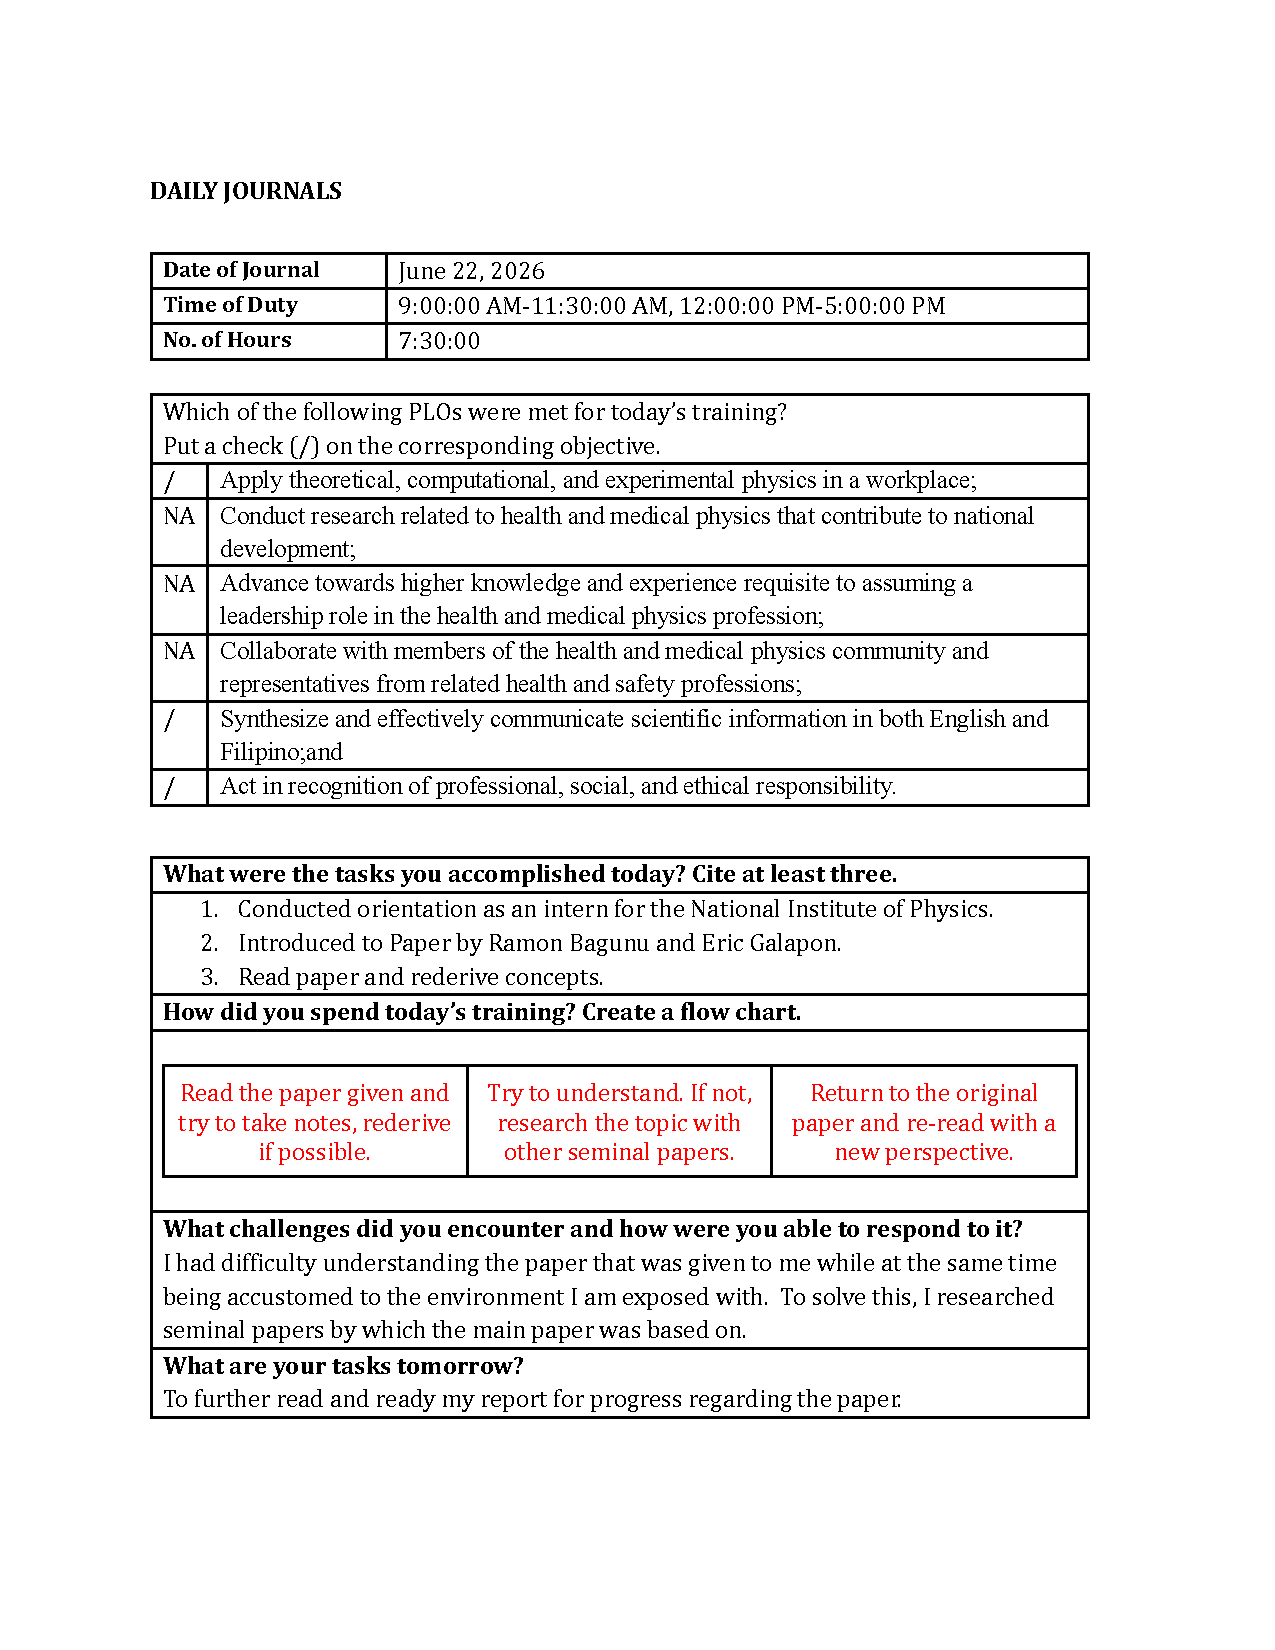
\includepdf[pages=-]{2.1 Daily Journals.pdf}
	\backgroundsetup{contents={
\includegraphics[width=\paperwidth,height=\paperheight]{Background 2.jpg}}}
	\newpage
	
	\newpage
	\subsection{OJT Program Review and Personal Professional Plan}
	\subsubsection{The OJT Program}
	As a new intern, stepping to the National Institute of Physics at the University of the Philippines Diliman has been a challenge for me. Sure, I have visited the area when I participated in the annual Proceedings of the Samahang Pisika ng Pilipinas conference conducted during the year 2025. However, stepping inside the actual laboratories by which scientific progress in numerous fields of physics was made was amazing to me. The internship started late, June 22, 2026, to be exact, due to the conduct of the 2026 Proceedings of the Samahang Pisika ng Pilipinas conference held at the CAS Annex Building, University of the Philippines Los Banos, of which I presented a poster presentation. The Deputy Director for Research and Extension, Dr. Lim, greeted and welcomed all of us warmly. A tour with the laboratory groups was conducted, inside the restricted portion of the institute. The room I called home for a short time was Room 204, also known as the Theory room, because it housed all of those who wanted to pursue research in Theoretical Physics. It was cold, filled with papers full of scratch equations, and whiteboards plastered over the walls. Fellow interns, Master’s students, and PhD students were writing on them, working on a niche problem such that each one admitted that they did not understand each other’s work. All except our supervisor, however, Dr. Eric A. Galapon. Originally, we were four, two people from University of the Philippines Manila (Me and Mr. River Villanueva), one from University of the Philippines Los Banos, and one from the Philippine Science High School Cagayan Valley Campus. Together, we spent the time to help each other grow accustomed to the environment we have been exposed with. At the start, we have been assigned papers by Dr. Galapon to study and produce the derivations within the paper. River and I had been assigned Sir Ramon Bagunu’s paper “Quantization of the Hamilton Equations of Motion.” The main goal was to reproduce the concepts and understand how such research is conducted in the Theory group, specifically the Quantum Physics subgroup. I finished the paper within the day, that is, a preliminary reading where I found the results interesting for the context given.  \\
	
	The actual derivations were the hardest part. I had been unfamiliar with the concepts introduced with the paper. Dr. Herbert Domingo did his best to prepare us on the possible concepts we would be exposed with. However, the unfamiliarity made me more excited to work on the paper and understand it but also at the same time be intimidated with it. I struggled with understanding and became insecure as, as compared to my peers who have done significant progress, I was stuck sometimes on some topics wondering “why would this condition be assumed,” or “why is this result used.” But due to the help of those very own peers and my supervisor who was always to consult upon when prompted, I was able to get past my insecurities and roadblock in the research. I also thought that in Theory, majority of the people would be preoccupied in their work to do anything else. But I soon learned, after taking late night stays in the laboratory due to my part-time job tutoring, that the people here are as sociable as me, lessening my worry that it wouldn’t be fun to pursue my further studies in physics. \\
	
	My time at the Theoretical Physics Group doesn’t end here. Temporarily, it does. But I have learned a lot. I learned to ask for help occasionally when I’m unfamiliar or having trouble, as extra perspectives could give significant influences in my own thinking. I may work more on being independent, but it wouldn’t hurt to also learn to rely on others to help me.
	
	\newpage
	
	\subsubsection{The Future of a BS Applied Physics Graduate}
	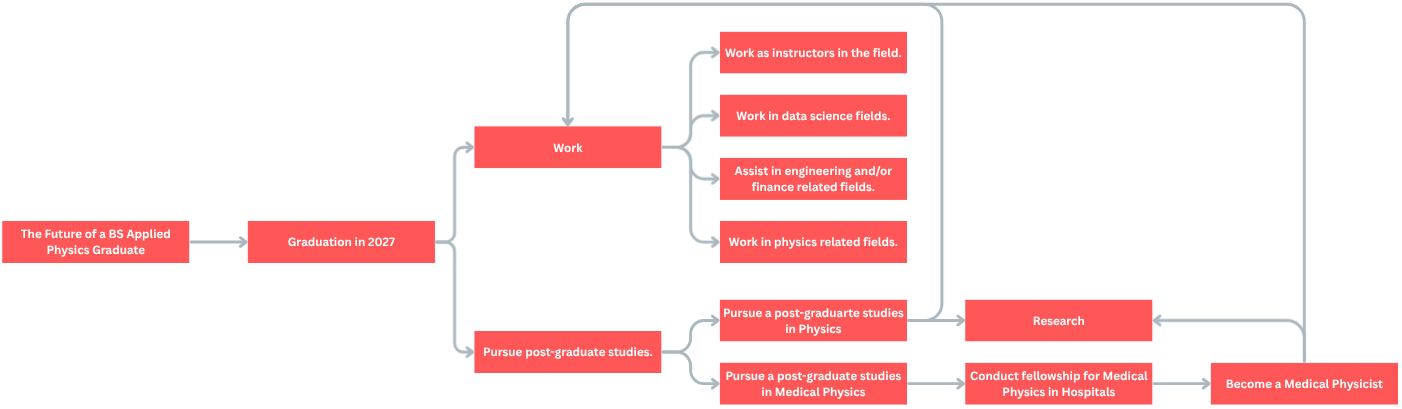
\includegraphics[width=\textwidth]{2.2 Future of BS Applied Physics.png}
	
	\subsection{Personal Professional Plan}
	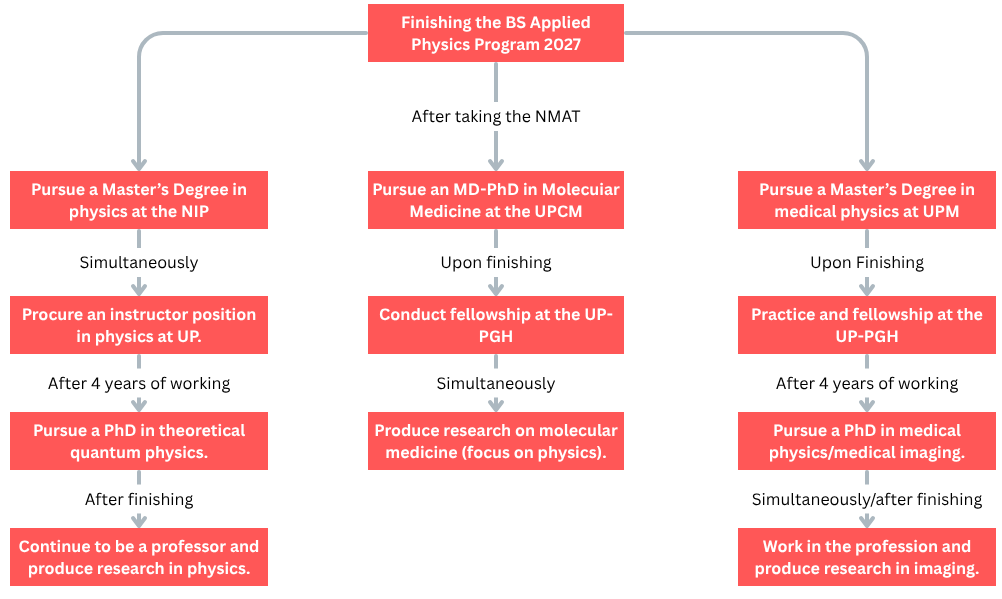
\includegraphics[width=\textwidth]{2.3 Personal Professional Plan.png}
	
	\newpage
	\vspace*{\fill}
	\section{Appendix}
	\vspace*{\fill}	
	\newpage
	
	\subsection{Completion Certificate}
	\noindent Supervisor has not accomplished this yet. This document is to follow.
	
	\subsection{Letter of Acceptance}
	\noindent Please see attached file on next page.
	
	\newpage
	\backgroundsetup{contents={}}
	
\includepdf{3.2 Acceptance Letter.pdf}
	\backgroundsetup{contents={
\includegraphics[width=\paperwidth,height=\paperheight]{Background 2.jpg}}}
	
	\subsection{Proposed Training and Design Schedule}
	Please see attached file on next page.
	
	\newpage
	\backgroundsetup{contents={}}
	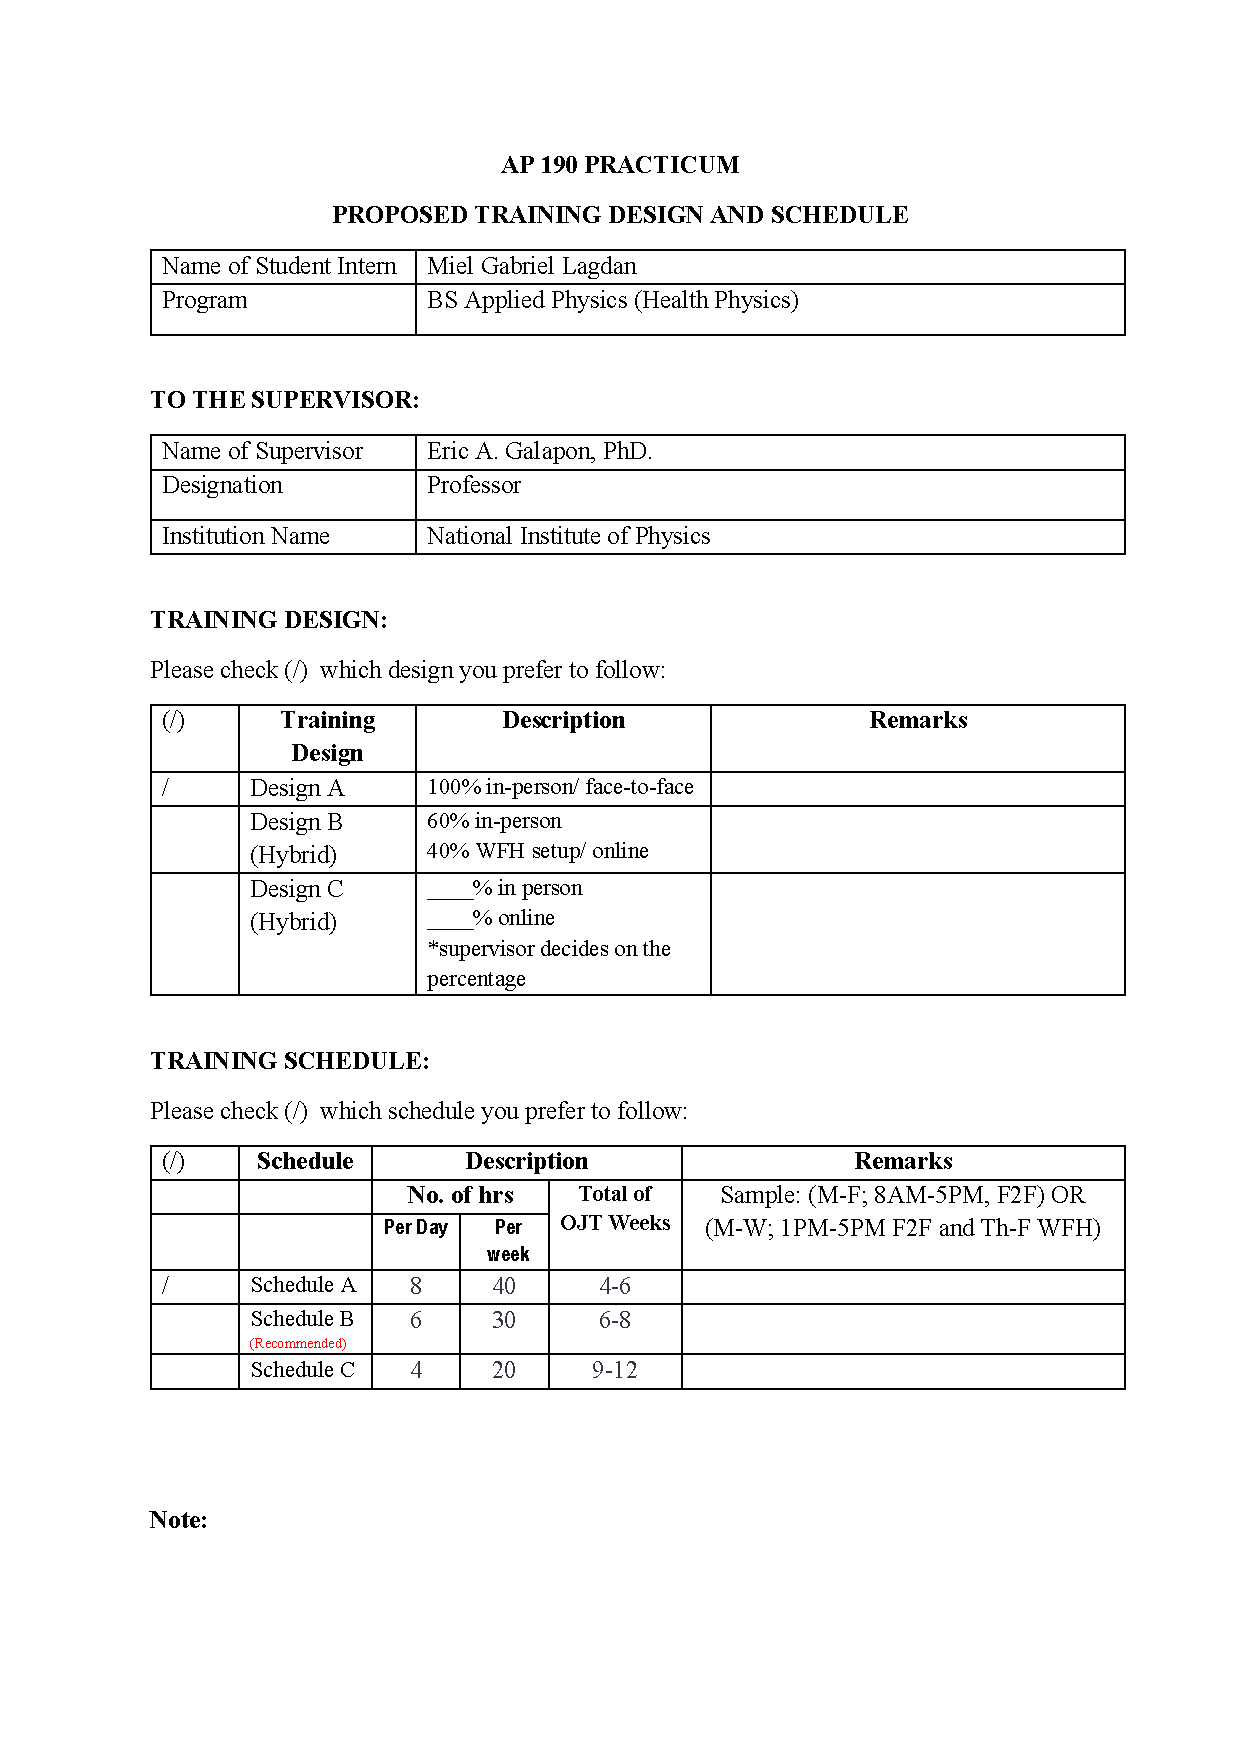
\includepdf[pages=-]{3.3 Proposed Training and Design Schedule.pdf}
	\backgroundsetup{contents={
\includegraphics[width=\paperwidth,height=\paperheight]{Background 2.jpg}}}
	\newpage
	
	\subsection{Supervisor’s Evaluation}
	\noindent Please see attached file on next page.
	
	\newpage
	\backgroundsetup{contents={}}
	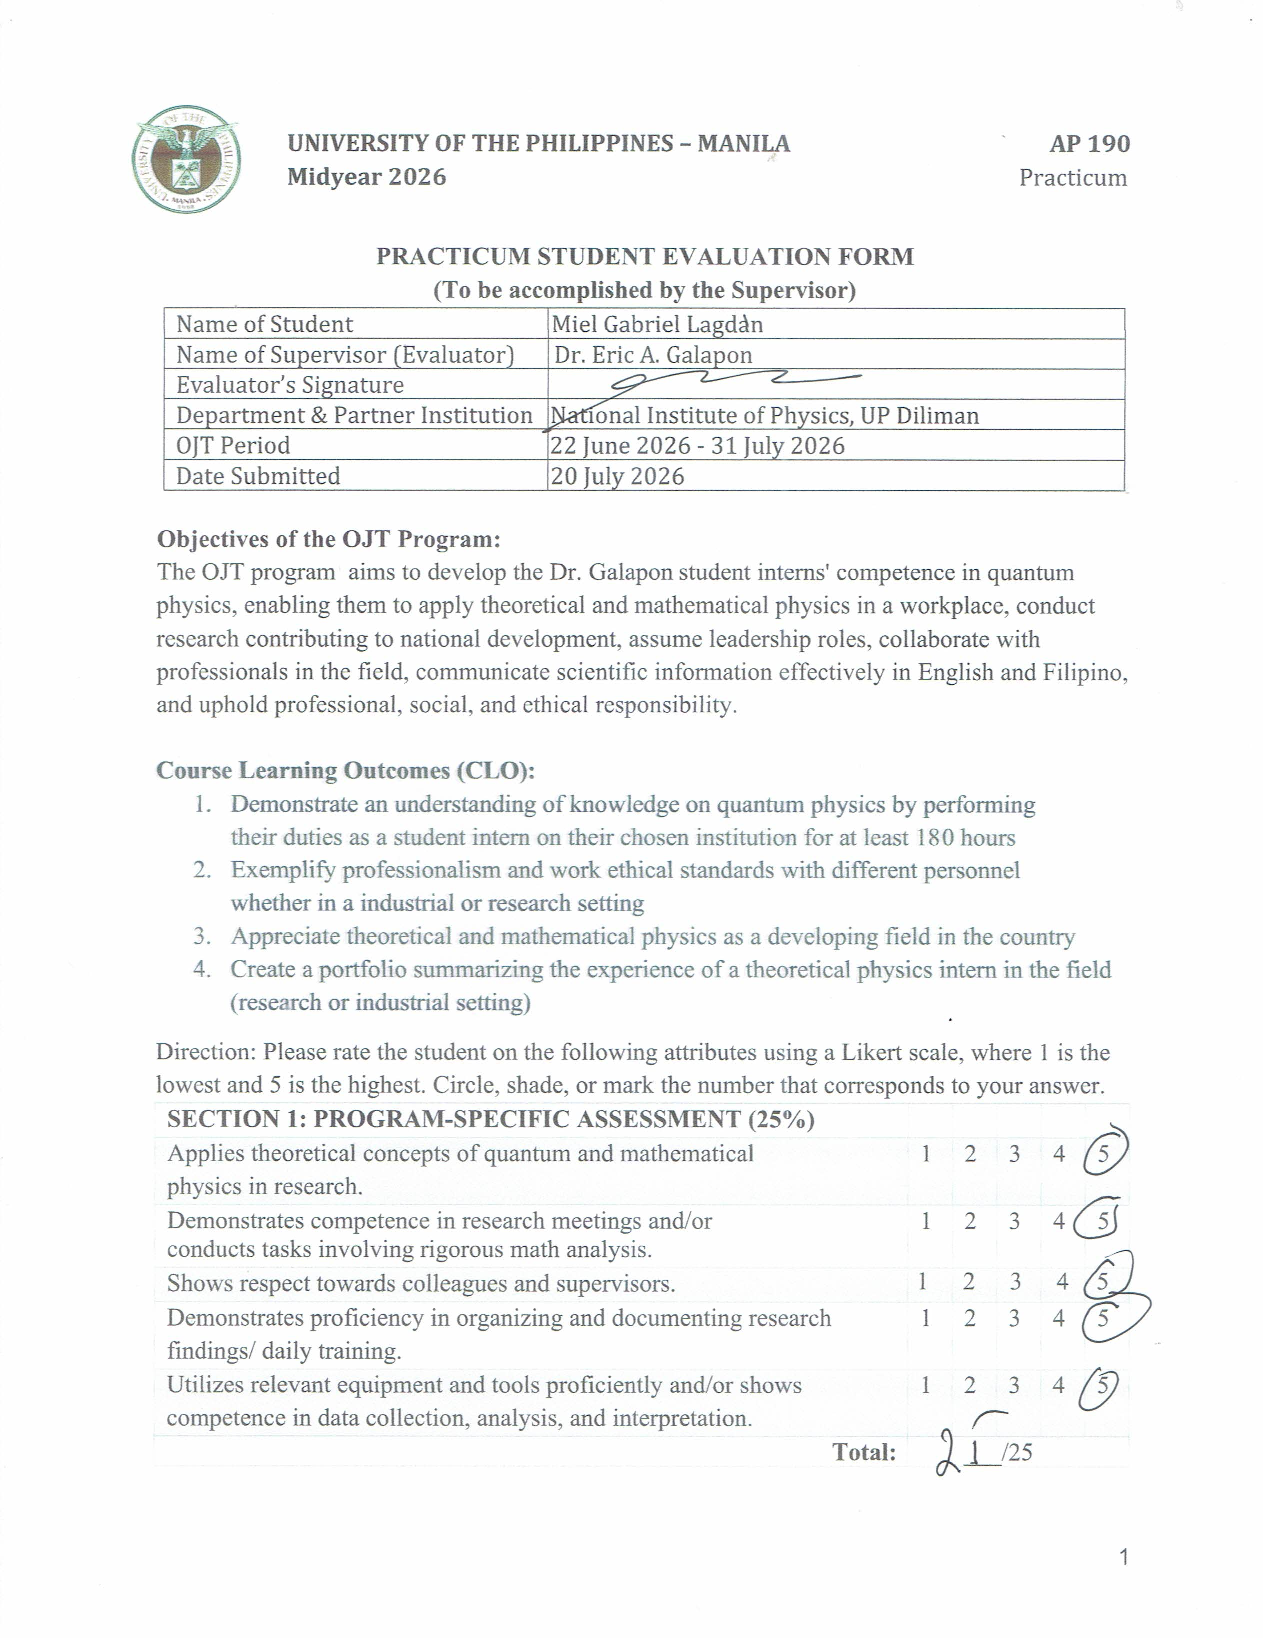
\includepdf[pages=-]{3.4 Supervisor's Evaluation.pdf}
	\backgroundsetup{contents={
\includegraphics[width=\paperwidth,height=\paperheight]{Background 2.jpg}}}
	\newpage
	
	\subsection{Pictures of Daily Journal}
	\begin{figure}[h]
		\begin{subfigure}{.5\textwidth}
			\centering
			\includegraphics[width=.8\linewidth]{Images/IMG_4442.png}
			\caption{June 22, 2026: Orientation Day}
			%\label{fig:sfig1}
		\end{subfigure}%
		\begin{subfigure}{.5\textwidth}
			\centering
			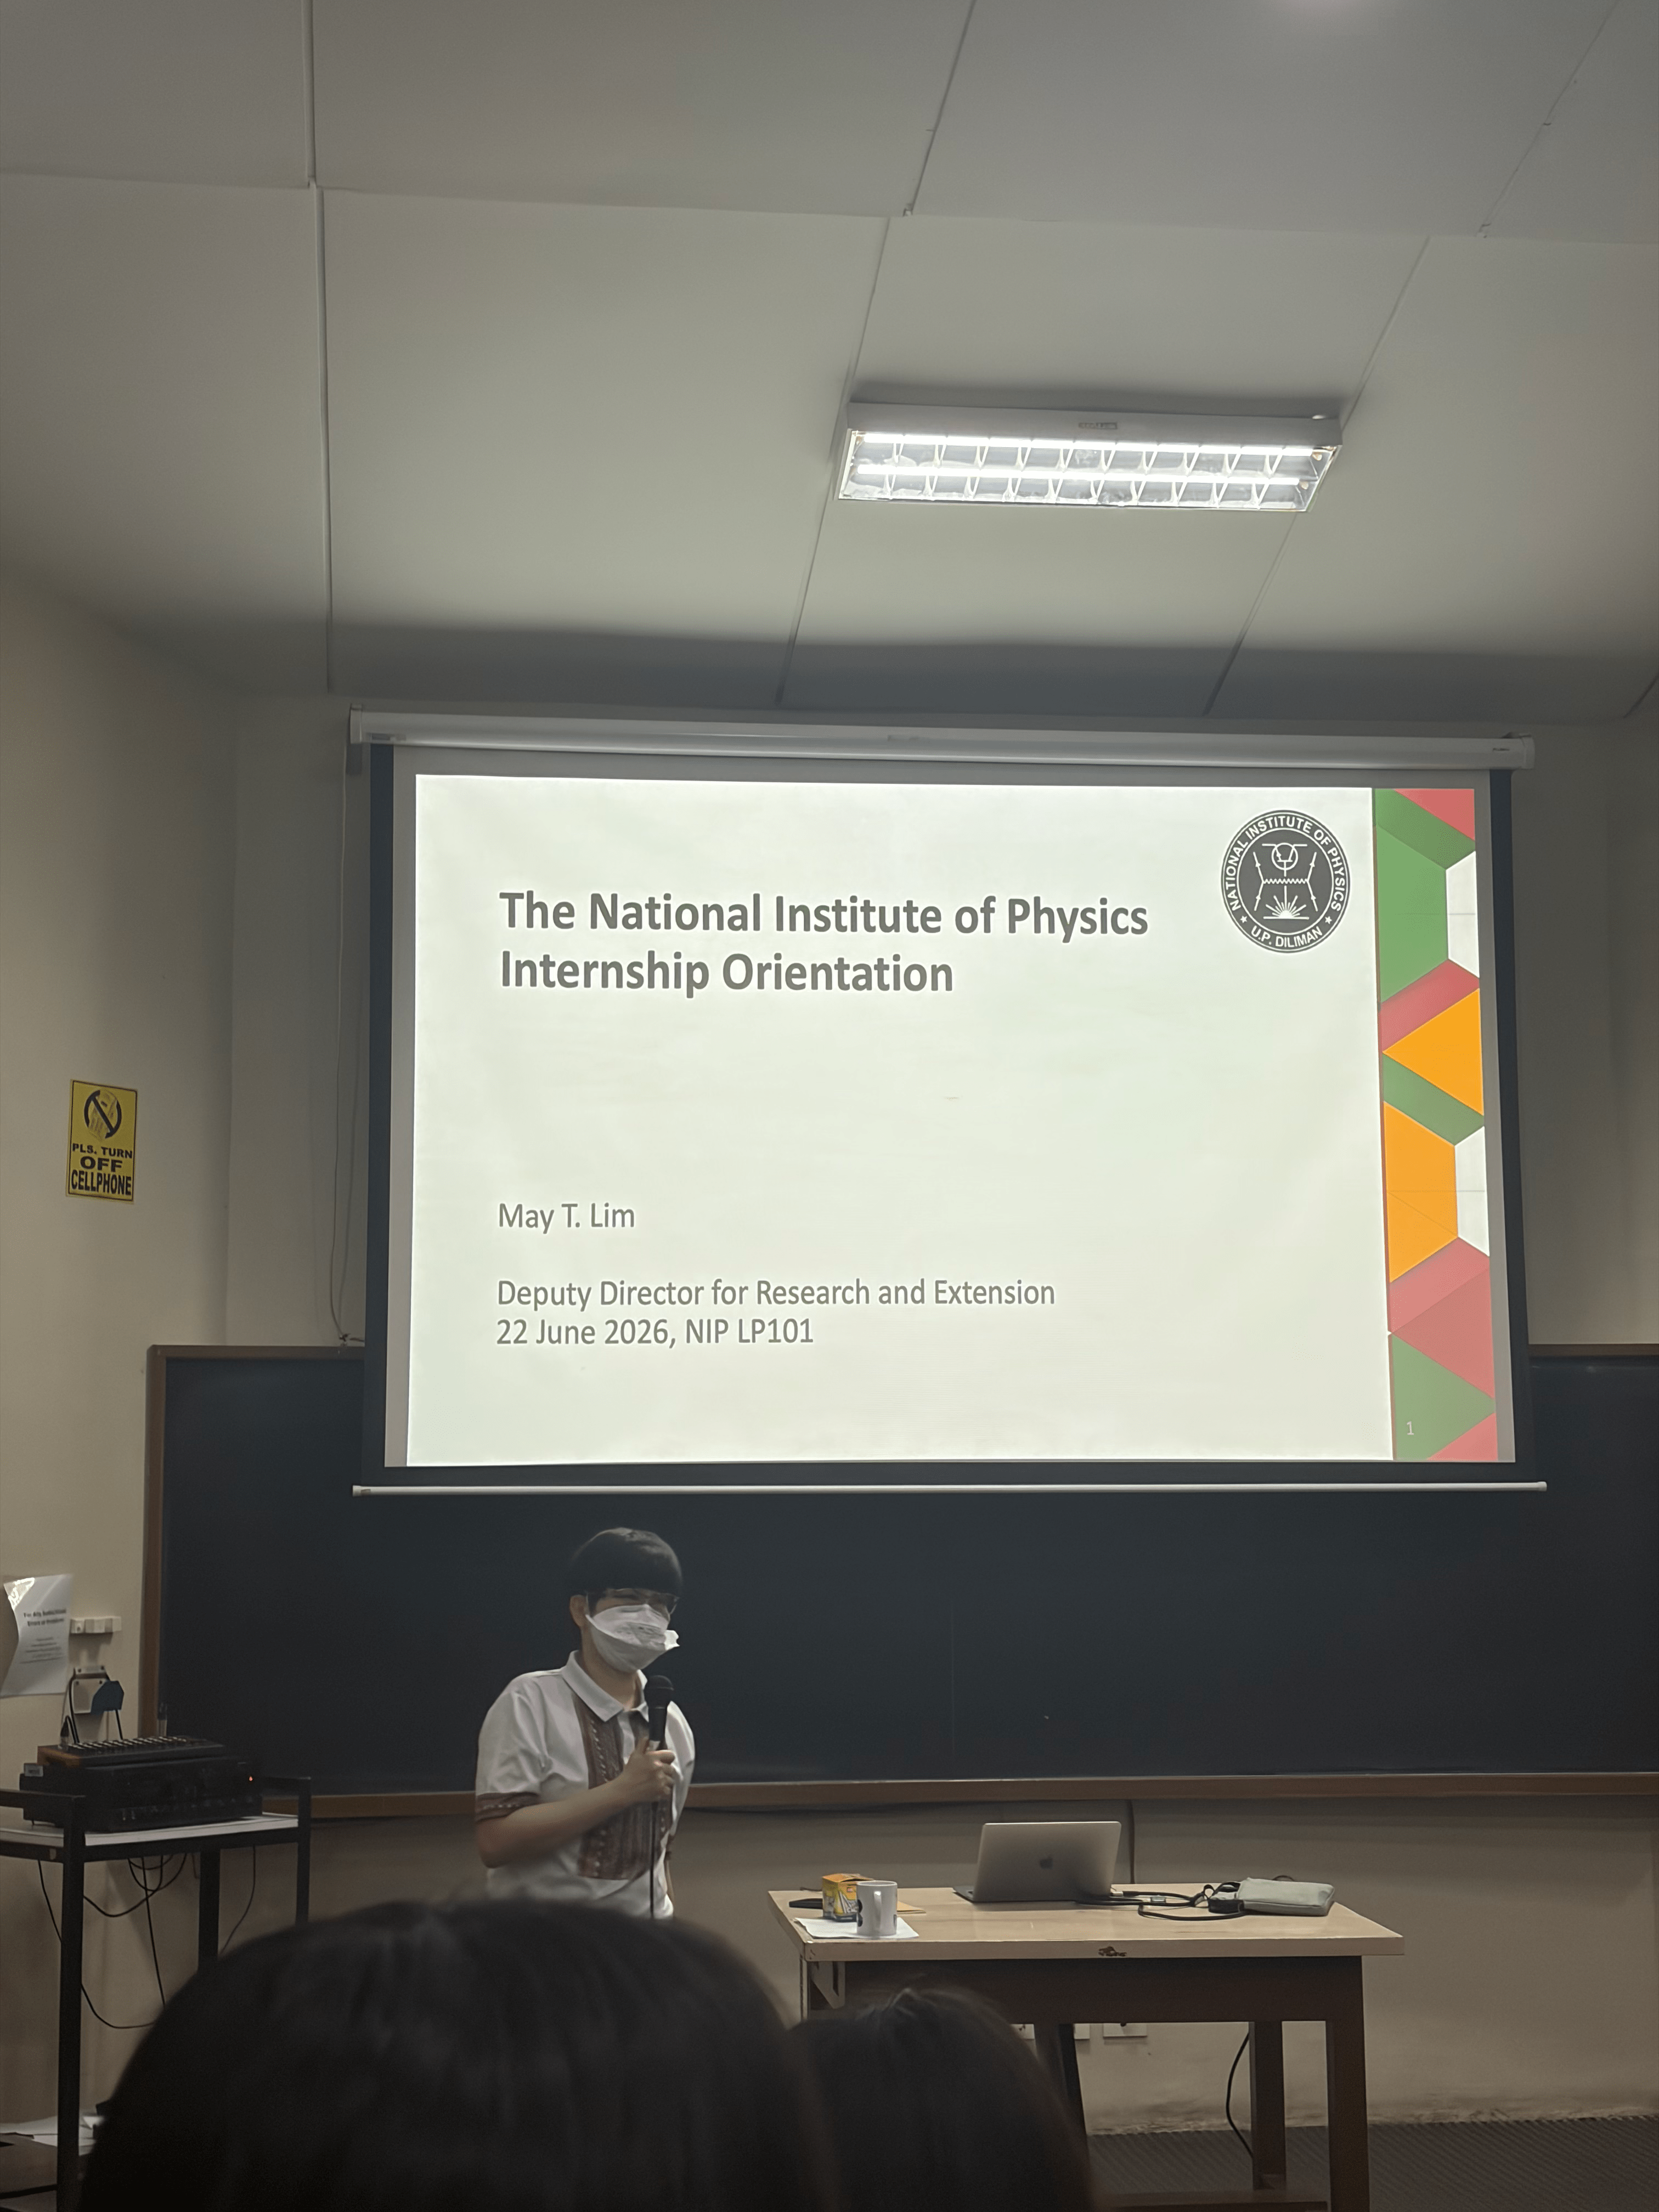
\includegraphics[width=.8\linewidth]{Images/IMG_4443.png}
			\caption{June 22, 2026: Orientation Day}
			%\label{fig:sfig2}
		\end{subfigure}
		\begin{subfigure}{.5\textwidth}
			\centering
			\includegraphics[width=.8\linewidth]{Images/IMG_5042.png}
			\caption{July 17, 2026: Paper Report}
			%\label{fig:sfig1}
		\end{subfigure}%
		\begin{subfigure}{.5\textwidth}
			\centering
			\includegraphics[width=.8\linewidth]{Images/IMG_5037.png}
			\caption{July 17, 2026: Paper Report}
			%\label{fig:sfig2}
		\end{subfigure}
		%\caption{plots of....}
		\label{fig:fig}
	\end{figure}
	\newpage
	
	\subsection{List of References Read During the Training}
	\vspace{0.5cm}
	{\noindent\textbf{MAIN PAPERS}:\\
\hrule
\begin{enumerate}
	\item Bagunu, R. J. C., \& Galapon, E. A. (2025). \textit{Quantization of the Hamilton equations of motion}. \textit{Physica Scripta}, \textit{100}(5), 055208. \url{https://doi.org/10.1088/1402-4896/adc047}
	
	\item Domingo, H. B., \& Galapon, E. A. (2015). \textit{Generalized Weyl transform for operator ordering: Polynomial functions in phase space}. \textit{Journal of Mathematical Physics}, \textit{56}(2). \url{https://doi.org/10.1063/1.4907561}
	
	\item Domingo, H. B. (2016). \textit{Algebra of Non-Weyl Operators and Quantization of Analytic and Non-Analytic Classical Functions}. [Unpublished dissertation]. University of the Philippines Diliman.
\end{enumerate}	

\noindent\textbf{RESOURCES}: \\
\hrule	
	\begin{enumerate}
		\item Olsen, P. A., Rennie, S. J., \& Goel, V. (2012). \textit{Efficient automatic differentiation of matrix functions}. In \textit{Lecture Notes in Computational Science and Engineering} (pp.~71--81). \url{https://doi.org/10.1007/978-3-642-30023-3_7}
		
		\item Muller, F. (1997). \textit{The equivalence myth of quantum mechanics---Part I}. \textit{Studies in History and Philosophy of Science Part B: Studies in History and Philosophy of Modern Physics}, \textit{28}(1), 35--61. \url{https://doi.org/10.1016/S1355-2198(96)00022-6}
		
		\item Cohen, L. (1976). \textit{Quantization problem and variational principle in the phase-space formulation of quantum mechanics}. \textit{Journal of Mathematical Physics}, \textit{17}(10), 1863--1866. \url{https://doi.org/10.1063/1.522807}
		
		\item Cohen, L. (1966). \textit{Generalized phase-space distribution functions}. \textit{Journal of Mathematical Physics}, \textit{7}(5), 781--786. \url{https://doi.org/10.1063/1.1931206}
		
		\item McCoy, N. H. (1932). \textit{On the Function in Quantum Mechanics Which Corresponds to a Given Function in Classical Mechanics}. \textit{Proceedings of the National Academy of Sciences}, \textit{18}(11), 674--676. \url{https://doi.org/10.1073/pnas.18.11.674}
		
		\item Moyal, J. E. (1949). \textit{Quantum mechanics as a statistical theory}. \textit{Mathematical Proceedings of the Cambridge Philosophical Society}, \textit{45}(1), 99--124. \url{https://doi.org/10.1017/S0305004100000487}
		
		\item Zachos, C. (2002). \textit{Deformation Quantization: Quantum Mechanics Lives and Works in Phase-Space}. \textit{International Journal of Modern Physics A}, \textit{17}(3), 297--316. \url{https://doi.org/10.1142/S0217751X02006079}
		
		\item Margenau, H., \& Hill, R. N. (1961). \textit{Correlation between Measurements in Quantum Theory}. \textit{Progress of Theoretical Physics}, \textit{26}(5), 722--738. \url{https://doi.org/10.1143/PTP.26.722}
		
		\item Daughaday, H., \& Nigam, B. P. (1965). \textit{Function in Quantum Mechanics Which Corresponds to a Given Function in Classical Mechanics}. \textit{Physical Review}, \textit{139}(5B), B1436--B1442. \url{https://doi.org/10.1103/PhysRev.139.B1436}
		
		\item Praxmeyer, L., \& Wódkiewicz, K. (2003). \textit{Hydrogen atom in phase space: The Kirkwood--Rihaczek representation}. \textit{Physical Review A}, \textit{67}(5). \url{https://doi.org/10.1103/PhysRevA.67.054502}
		
		\item Kirkwood, J. (1933). \textit{Quantum Statistics of Almost Classical Assemblies}. \textit{Physical Review}, \textit{44}(1), 31--37. \url{https://doi.org/10.1103/PhysRev.44.31}
		
		\item Fan, H., Yuan, H., Cai, G., \& Jiang, N. (2011). \textit{Operators' ordering: from Weyl ordering to normal ordering}. \textit{Science China Physics, Mechanics and Astronomy}, \textit{54}(8), 1394--1397. \url{https://doi.org/10.1007/s11433-011-4404-z}
		
		\item Fan, H. (1992). \textit{Weyl ordering quantum mechanical operators by virtue of the IWWP technique}. \textit{Journal of Physics A: Mathematical and General}, \textit{25}(11), 3443--3447. \url{https://doi.org/10.1088/0305-4470/25/11/043}
		
		\item Tang, X., Sun, Y., \& Su, H. (2010). \textit{Weyl ordering symbol method for studying Wigner function of the damping field}. \textit{International Journal of Theoretical Physics}, \textit{49}(9), 2016--2027. \url{https://doi.org/10.1007/s10773-010-0385-3}
		
		\item Cohen, L. (2012). \textit{The Weyl Operator and its Generalization}. \url{https://doi.org/10.1007/978-3-0348-0294-9}
		
		\item Qian, M., \& Xu, P. (1988). \textit{Generalized Weyl transformation}. \textit{Acta Mathematicae Applicatae Sinica English Series}, \textit{4}(3), 275--288. \url{https://doi.org/10.1007/BF02006225}
		
		\item De Gosson, M. A., \& Luef, F. (2015). \textit{Born--Jordan pseudodifferential calculus, BOPP operators and deformation quantization}. \textit{Integral Equations and Operator Theory}, \textit{84}(4), 463--485. \url{https://doi.org/10.1007/s00020-015-2273-y}
		
		\item Neudecker, H. (1969). \textit{Some Theorems on Matrix Differentiation with Special Reference to Kronecker Matrix Products}. \textit{Journal of the American Statistical Association}, \textit{64}(327), 953--963. \url{https://doi.org/10.1080/01621459.1969.10501027}
		
		\item Bender, C. M., \& Dunne, G. V. (1989). \textit{Exact solutions to operator differential equations}. \textit{Physical Review D}, \textit{40}(8), 2739.
		
		\item Fujii, K., \& Suzuki, T. (2004). \textit{A New Symmetric Expression of Weyl Ordering}. \textit{Modern Physics Letters A}, \textit{19}(11), 827--840. \url{https://doi.org/10.1142/S021773230401374X}
		
		\item Fan, H., \& Fan, Y. (2002). \textit{Weyl Ordering for Entangled State Representation}. \textit{International Journal of Modern Physics A}, \textit{17}(5), 701--708. \url{https://doi.org/10.1142/S0217751X02003257}
		
		\item Gelfand, I. M., \& Fairlie, D. B. (1991). \textit{The algebra of Weyl symmetrised polynomials and its quantum extension}. \textit{Communications in Mathematical Physics}, \textit{136}(3), 487--499. \url{https://doi.org/10.1007/BF02099070}
		
		\item Bargellini, A. E., \& Ritelli, D. (2026). \textit{An elementary approach to Euler's reflection formula and its role in the infinite product of the sine function and the Basel problem}. \textit{Foundations}, \textit{6}(2), 14. \url{https://doi.org/10.3390/foundations6020014}
		
		\item Fedak, W. A., \& Prentis, J. J. (2009). \textit{The 1925 Born and Jordan paper ``On quantum mechanics''}. \textit{American Journal of Physics}, \textit{77}(2), 128--139. \url{https://doi.org/10.1119/1.3009634}
		
		\item Born, M., \& Jordan, P. (1925). \textit{Zur Quantenmechanik}. \textit{The European Physical Journal A}, \textit{34}(1), 858--888. \url{https://doi.org/10.1007/BF01328531}
		
		\item Suzuki, M. (1999). \textit{General Formulation of Quantum Analysis}. \textit{Reviews in Mathematical Physics}, \textit{11}(2), 243--265. \url{https://doi.org/10.1142/S0129055X9900009X}
	\end{enumerate}}
	
	\subsection{Abstract of Proposed Thesis}
	\vspace{0.5cm}
	\begin{mdframed}
	{\Large\textbf{Quantization Ambiguities in Entanglement-Enhanced Interferometric Phase Generators}}\\
	Miel Gabriel Lagdan, Herbert B. Domingo \\
	\vspace{0.25cm}
	
	\noindent Measurements involving photons are classically limited by the shot-noise limit. Entanglement in nonlinear interferometers enables these systems to approach or surpass the Heisenberg limit. However, the quantization of phase generators is plagued by ambiguities arising from different operator-ordering prescriptions (e.g., Weyl, Born-Jordan, and simplest symmetrization). This thesis investigates these ambiguities by deriving and comparing the phase sensitivities of entanglement-enhanced interferometric phase generators constructed under various ordering rules. Implications for quantum metrology in nonlinear media are discussed.
	\end{mdframed}
	
	\subsection{Resume}
	\noindent Please see attached file on next page.
	\newpage
	
	\backgroundsetup{contents={}}
	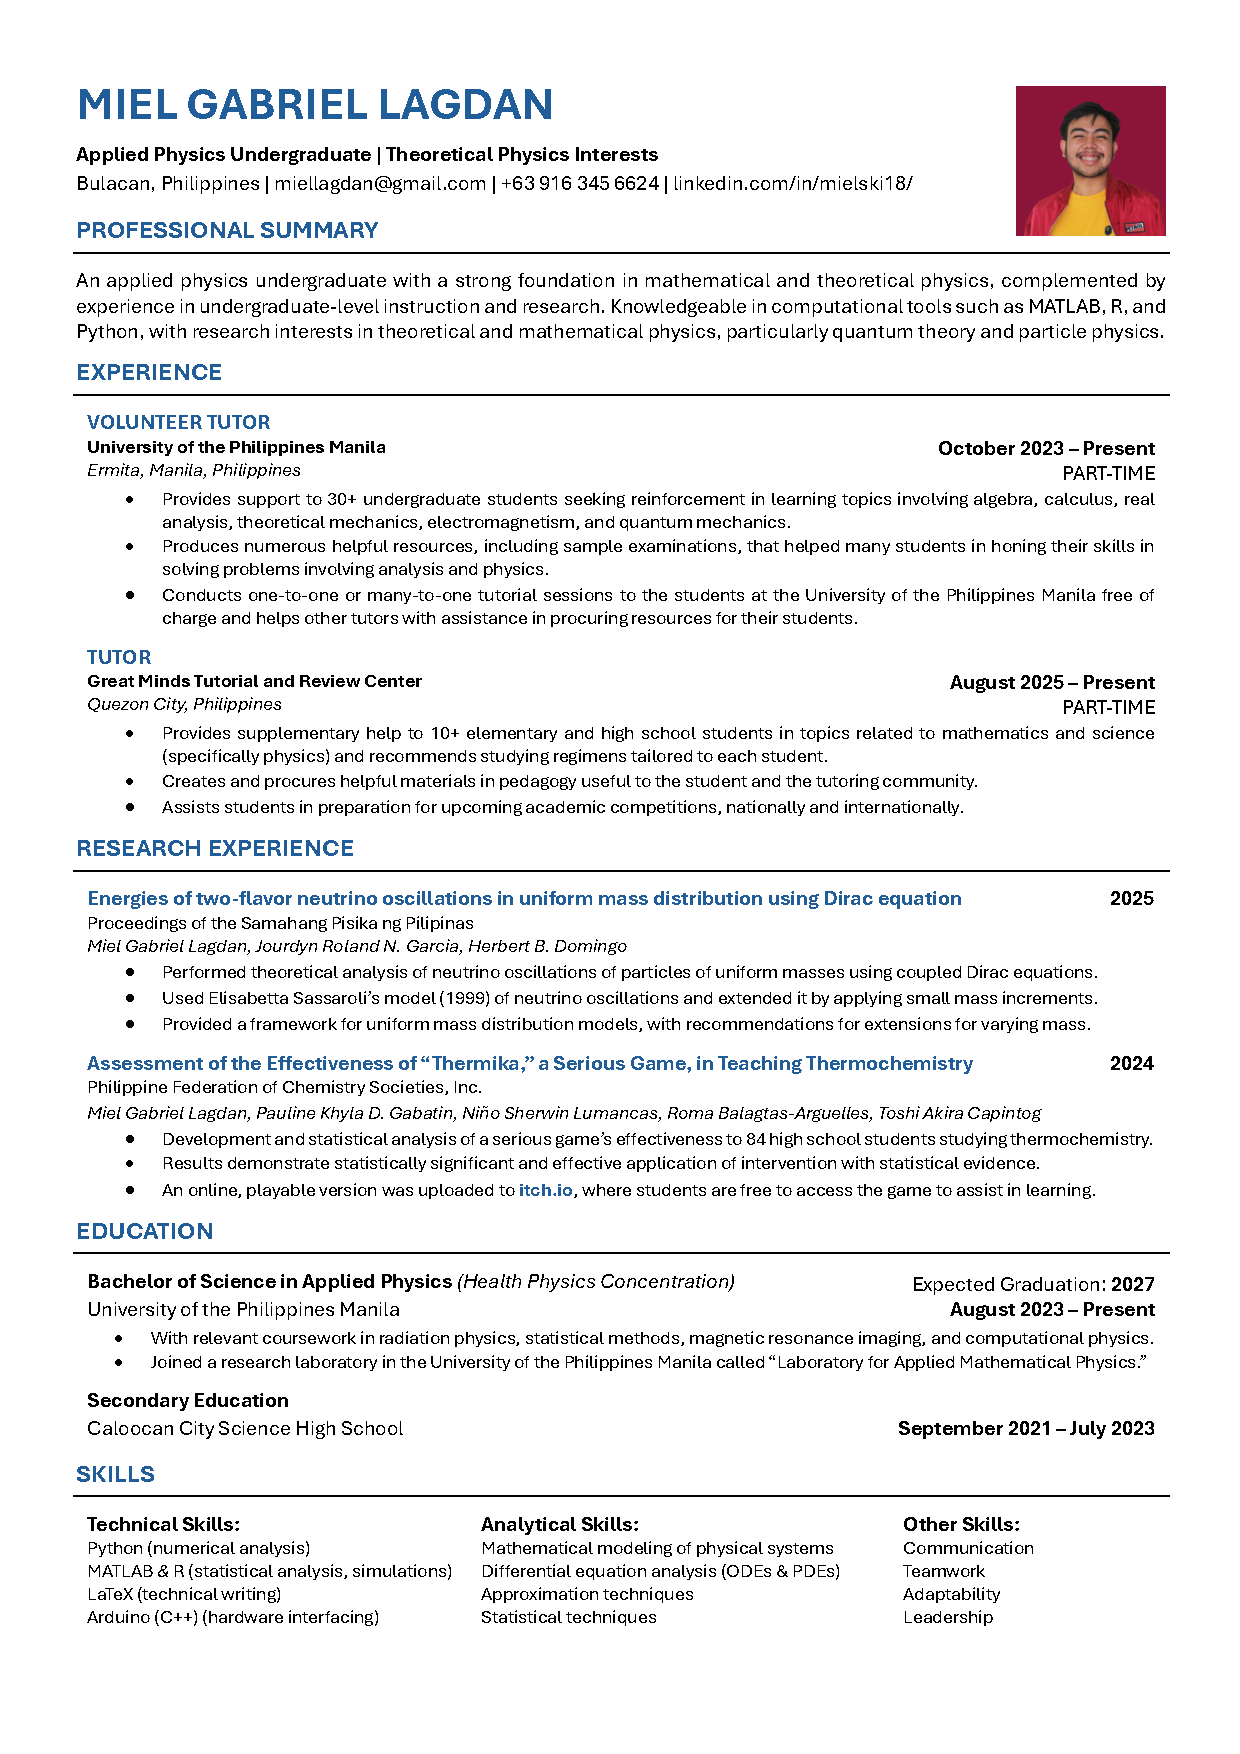
\includepdf{3.7 Resume.pdf}
	\backgroundsetup{contents={
\includegraphics[width=\paperwidth,height=\paperheight]{Background 2.jpg}}}
	
	\subsection{OUTPUT: Analysis of Paper (Bagunu \& Galapon)}\label{sec:output1}
	\noindent Please see linked file to research repository. \\
	\begin{mdframed}
		\noindent Link to Repository: \href{https://github.com/mielski2185/tp-quant-rs-1/blob/2650112dfcc6634a3ba3a4a2c2bba0acb26d5b76/Research%20Analysis/%5B2026-06-22%5D%20Quantization%20of%20the%20Hamilton%20Equations%20of%20Motion.pdf}{Analysis Paper (Bagunu and Galapon)}
	\end{mdframed}
	%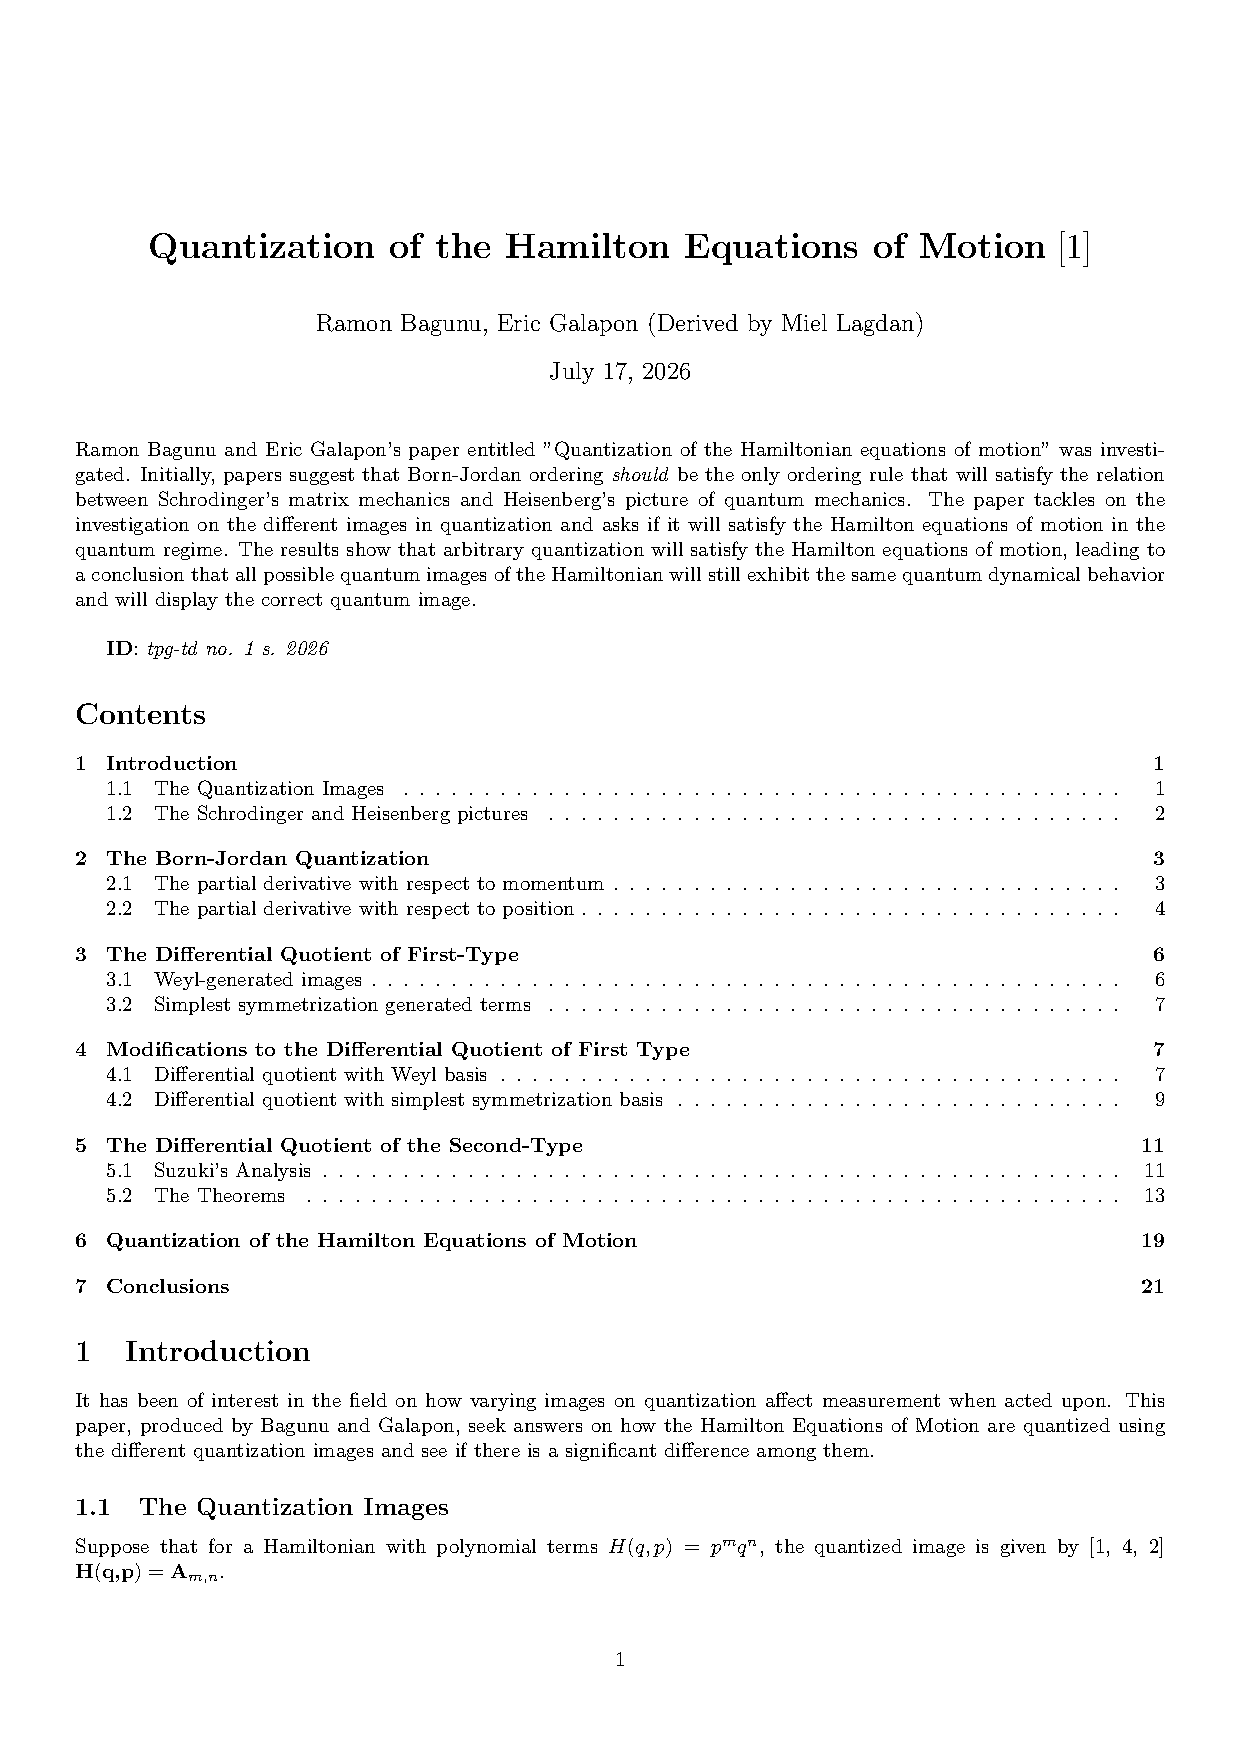
\includepdf[pages=-]{3.8 Report (BG).pdf}
	
	\subsection{Time Card}
	\noindent Please see attached file on next page.
	\newpage
	
	\backgroundsetup{contents={}}
	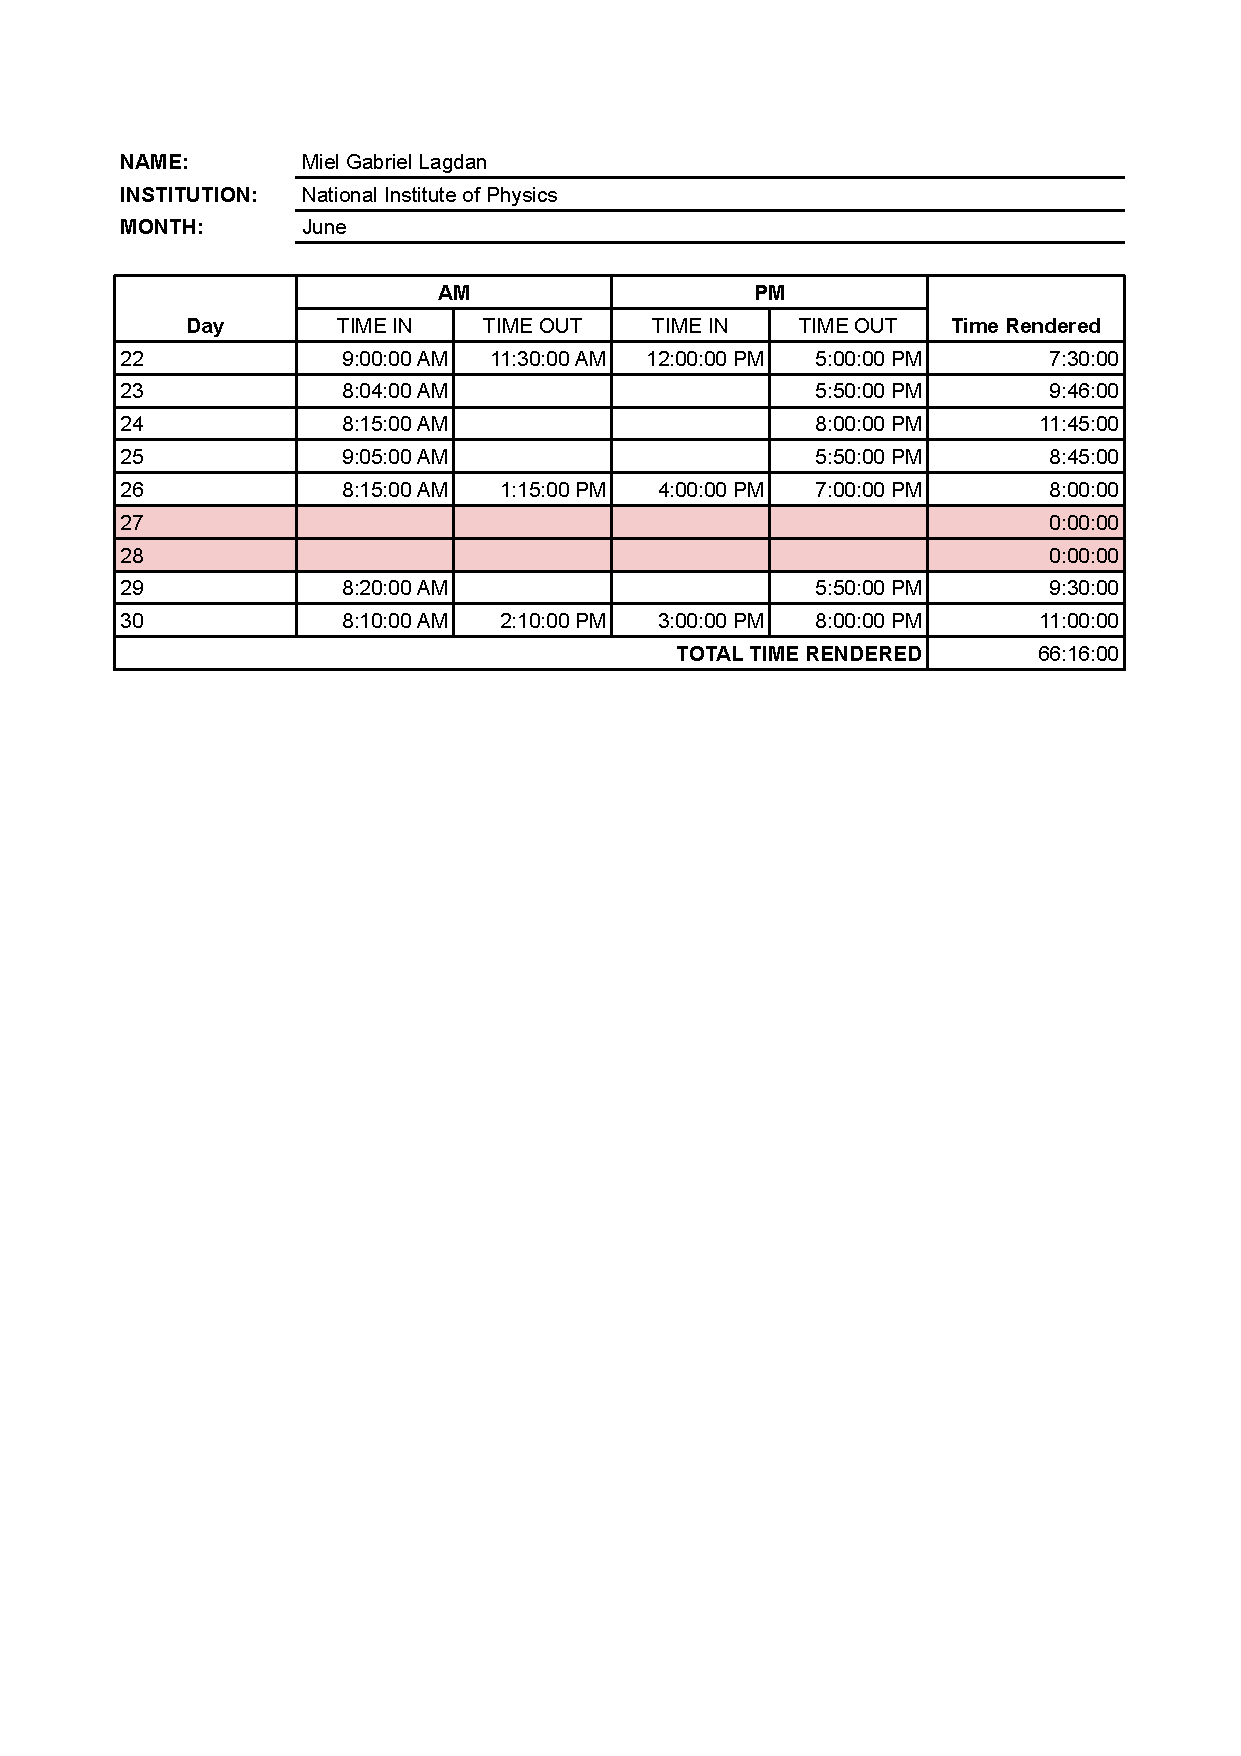
\includepdf[pages=-]{3.9 Time Card.pdf}
	\backgroundsetup{contents={
\includegraphics[width=\paperwidth,height=\paperheight]{Background 2.jpg}}}
\end{document}
